% =====================================================================
%  Perceiver --- Sintesi Teorica (ripasso visuale per l'esame)
%  Estratto e distillato dalla Sezione 1 di appunti_ml.tex (pp. 5-87).
%  Documento standalone: compilare con  pdflatex perceiver_teoria.tex
% =====================================================================
\documentclass[11pt]{article}

\usepackage[T1]{fontenc}
\usepackage[utf8]{inputenc}
\usepackage{lmodern}
\IfFileExists{microtype.sty}{\usepackage{microtype}}{}
\usepackage[dvipsnames]{xcolor}
\usepackage[a4paper,margin=2.4cm,headheight=26pt,headsep=9pt]{geometry}
\usepackage{amsmath,amssymb}
\usepackage{graphicx}
\usepackage{booktabs}
\usepackage{array}
\usepackage{enumitem}
\usepackage{tcolorbox}
\tcbuselibrary{skins,breakable}
\usepackage{titlesec}
\usepackage{needspace}
\usepackage{fancyhdr}
\usepackage{hyperref}

\setcounter{secnumdepth}{2}
\setcounter{tocdepth}{2}

% ---- Colori ----
\definecolor{seccolor}{HTML}{1a237e}
\definecolor{linkblue}{HTML}{1565c0}
\definecolor{ideagreen}{HTML}{1b5e20}
\definecolor{escolor}{HTML}{00695c}
\definecolor{boxbg}{HTML}{f5f5f5}
\definecolor{boxframe}{HTML}{bdbdbd}
\definecolor{tldrbg}{HTML}{fff8e1}
\definecolor{tldrframe}{HTML}{f9a825}

% ---- Nomi in italiano ----
\renewcommand{\figurename}{Figura}
\renewcommand{\tablename}{Tabella}
\renewcommand{\contentsname}{Indice}

% ---- Liste e paragrafi ----
\setlist{itemsep=2pt, parsep=1pt, topsep=4pt}
\setlength{\parindent}{0pt}
\setlength{\parskip}{6pt plus 2pt minus 1pt}
\raggedbottom

% ---- Stile titoli ----
\titleformat{\section}{\needspace{8\baselineskip}\Large\bfseries\color{seccolor}}{\thesection}{0.7em}{}[\vspace{2pt}\titlerule]
\titleformat{\subsection}{\needspace{6\baselineskip}\large\bfseries\color{seccolor!85!black}}{\thesubsection}{0.6em}{}
\titlespacing*{\section}{0pt}{1.5em}{0.6em}
\titlespacing*{\subsection}{0pt}{1.1em}{0.4em}

% ---- Box: formula (blu) ----
\newtcolorbox{formulabox}[1][]{
  colback=blue!3, colframe=seccolor!50, boxrule=0.5pt,
  arc=3pt, left=8pt, right=8pt, top=6pt, bottom=6pt, breakable, #1}

% ---- Box: nota a margine (grigio) ----
\newtcolorbox{notabox}[1][]{
  colback=boxbg, colframe=boxframe, boxrule=0.4pt,
  arc=2pt, left=6pt, right=6pt, top=4pt, bottom=4pt,
  breakable, fontupper=\small, #1}

% ---- Box: idea chiave da memorizzare (verde) ----
\newtcolorbox{ideabox}[1][]{
  colback=ideagreen!5, colframe=ideagreen!60, boxrule=0.9pt,
  coltitle=white, arc=3pt, left=8pt, right=8pt, top=6pt, bottom=6pt,
  breakable, #1}

% ---- Box: esempio numerico svolto (verde acqua) ----
\newtcolorbox{esempiobox}[1][]{
  colback=escolor!6, colframe=escolor!55, boxrule=0.7pt,
  coltitle=white, arc=3pt, left=8pt, right=8pt, top=6pt, bottom=6pt,
  breakable, fontupper=\small, #1}

% ---- Box: ripasso esame (ambra) ----
\newtcolorbox{esamebox}[1][]{
  colback=tldrbg, colframe=tldrframe!88!black, boxrule=1pt,
  coltitle=white, arc=3pt, left=8pt, right=8pt, top=6pt, bottom=6pt,
  breakable, #1}

% ---- Box: "In breve" a inizio sezione (navy) ----
\newtcolorbox{brevebox}[1][]{
  colback=seccolor!5, colframe=seccolor!75, boxrule=0.9pt,
  coltitle=white, arc=3pt, left=8pt, right=8pt, top=5pt, bottom=5pt,
  breakable, fontupper=\small, #1}

% =====================================================================
%  Striscia-pipeline ripetuta in cima a OGNI pagina (header)
%  \stage{n} (dopo ogni titolo) imposta la fase evidenziata.
%   1 Input  2 Fourier  3 Latenti  4 Cross-Att  5 Latent Transf.
%   6 xT     7 Pooling   0 = nessuna evidenziata
% =====================================================================
\newcommand{\curstage}{0}
\newcommand{\stage}[1]{\gdef\curstage{#1}}
\newcommand{\hchip}[2]{%
  \setlength{\fboxsep}{2.6pt}%
  \ifnum\curstage=#1\relax
    \colorbox{seccolor}{\textcolor{white}{\bfseries #2}}%
  \else
    \colorbox{seccolor!8}{\textcolor{seccolor!55}{#2}}%
  \fi}
\newcommand{\harr}{{\fontsize{7}{7}\selectfont\;\textcolor{seccolor!45}{$\rightarrow$}\;}}
\newcommand{\pipelinestrip}{%
  {\sffamily\fontsize{6.6}{8}\selectfont
   \hchip{1}{Input}\harr\hchip{2}{Fourier}\harr\hchip{3}{Latenti}\harr%
   \hchip{4}{Cross-Att}\harr\hchip{5}{Latent Transf.}\harr%
   \hchip{6}{$\times T$}\harr\hchip{7}{Pooling}}}
\pagestyle{fancy}
\fancyhf{}
\fancyhead[C]{\pipelinestrip}
\fancyfoot[C]{\small\thepage}
\renewcommand{\headrulewidth}{0.4pt}
\renewcommand{\footrulewidth}{0pt}

\hypersetup{
  colorlinks=true,
  linkcolor=seccolor!70!black,
  urlcolor=linkblue,
  pdftitle={Perceiver --- Sintesi Teorica}}

\title{\textbf{\color{seccolor} Perceiver --- Sintesi Teorica}\\[4pt]
  \large Ripasso visuale per l'esame di Deep Learning}
\author{}
\date{}

\begin{document}
\maketitle
\stage{0}
\vspace{-2.2em}

Questo documento è una sintesi della \textbf{Sezione 1 (\emph{Perceiver})} degli appunti completi (\texttt{appunti\_ml.tex}, pp.~5--87). Raccoglie \textbf{la teoria} dell'architettura --- l'idea di fondo, i blocchi, il forward pass \emph{passo per passo} con le forme delle matrici e gli esempi numerici, il \emph{perché} di ogni scelta. È escluso solo il backward pass (le derivazioni dei gradienti: puro calcolo, non teoria).

\begin{notabox}
\textbf{Come usare questo documento.} In cima a ogni pagina trovi la \textbf{striscia-pipeline}: le $7$ fasi del Perceiver, con evidenziata in blu quella di cui tratta la pagina. A inizio di ogni sezione un box \textbf{``In breve''} ne ricapitola il contenuto. I box \textbf{verdi} sono le idee-chiave da memorizzare, i box \textbf{verde acqua} esempi numerici svolti.
\end{notabox}

\begin{esamebox}[title={\textbf{Il Perceiver in 60 secondi}}]
Il \textbf{Perceiver} (Jaegle et al., 2021) è un'architettura \textbf{general-purpose}: processa qualsiasi modalità (immagini, audio, video, point cloud) con un \emph{unico} modello, senza componenti specifici per il dominio. Risolve il collo di bottiglia quadratico $O(M^2)$ della self-attention introducendo un \textbf{latent array} di dimensione fissa $N \ll M$: una \textbf{cross-attention} comprime l'input enorme in questo spazio latente (costo $O(MN)$), poi un \textbf{latent transformer} lo raffina con self-attention profonda (costo $O(N^2)$). Il blocco viene ripetuto $T$ volte con \textbf{weight sharing} $\Rightarrow$ il modello è di fatto un \textbf{RNN} che raffina progressivamente i latenti rileggendo lo stesso input.

\smallskip
\centering\small\ttfamily
Input $\to$ Byte Array $+$ Fourier PE $\to$ [\,Cross-Att $\to$ Latent Transformer\,]$\times T$ $\to$ Pooling $\to$ Logits
\end{esamebox}

{\small\tableofcontents}
\clearpage

% =====================================================================
\section{Il problema: la complessità quadratica}
\stage{0}
% =====================================================================

\begin{brevebox}[title={\textbf{In breve}}]
\textbf{CNN}: scalabili ($O(MKL)$) ma servono architetture specializzate per ogni dominio. \textbf{Transformer}: generali ma costano $O(M^2)$. \textbf{Perceiver}: generale \emph{e} scalabile, grazie a un \textbf{latent bottleneck} $N \ll M$ --- la complessità passa da $O(M^2)$ a $O(MN) + O(N^2)$.
\end{brevebox}

Prima del Perceiver, due famiglie di reti dominavano, ognuna con un pregio e un difetto opposti:

\begin{itemize}
\item \textbf{CNN} --- \emph{scalabili} (costo $O(MKL)$, lineare nel numero di input $M$) ma richiedono un'\textbf{architettura specializzata per ogni dominio} (convoluzioni 2D per le immagini, 1D per l'audio, \dots): poco generali.
\item \textbf{Transformer} --- \emph{generali} (un solo meccanismo, l'attention, per qualsiasi dato) ma la self-attention costa $O(M^2)$: ogni elemento confronta sé stesso con tutti gli altri. Su input grandi diventa impraticabile --- un'immagine ImageNet $224\times224$ ha $M = 50\,176$ pixel, cioè una matrice di attenzione da $\sim2.5$ miliardi di entry.
\end{itemize}

Il Perceiver \textbf{unisce il meglio dei due}: la \emph{generalità} del Transformer e la \emph{scalabilità} delle CNN. La chiave è un \textbf{latent bottleneck} --- un collo di bottiglia di dimensione fissa attraverso cui far passare l'input.

\begin{center}
\begin{tabular}{@{}llll@{}}
\toprule
\textbf{Famiglia} & \textbf{Costo attention} & \textbf{Scalabilità} & \textbf{Generalità} \\
\midrule
CNN          & $O(MKL)$ --- lineare        & alta  & \textbf{bassa} (arch.\ per dominio) \\
Transformer  & $O(M^2)$ --- \textbf{quadratico} & \textbf{bassa} & alta \\
\textbf{Perceiver} & $O(MN)+O(N^2)$ --- lineare & \textbf{alta} & \textbf{alta} \\
\bottomrule
\end{tabular}
\end{center}

\begin{formulabox}[title={\textbf{Riduzione della complessità}}]
\[
\underbrace{O(M^2)}_{\text{Self-attention (Transformer)}}
\;\;\longrightarrow\;\;
\underbrace{O(MN)}_{\text{Cross-attention}} \;+\; \underbrace{O(N^2)}_{\text{Self-attention latente}}
\]
Con $N = 512$ e $M = 50\,176$ il fattore di riduzione è $\approx 100\times$. Poiché $N$ è \emph{fisso}, il costo cresce solo \emph{linearmente} in $M$.
\end{formulabox}

\begin{ideabox}[title={\textbf{Idea chiave}}]
Un solo modello per tutte le modalità, a costo \textbf{lineare} nell'input. Il prezzo da pagare: l'input va prima \emph{compresso} in $N \ll M$ latenti. Tutto il resto dell'architettura discende da questa scelta.
\end{ideabox}

% =====================================================================
\section{L'idea centrale: dalla self- alla cross-attention}
\stage{0}
% =====================================================================

\begin{brevebox}[title={\textbf{In breve}}]
\textbf{Self-attention}: $Q,K,V$ vengono tutti dallo stesso input $\Rightarrow$ matrice di attenzione $M \times M$. \textbf{Cross-attention}: $Q$ viene dai \emph{latenti}, $K,V$ dall'\emph{input} $\Rightarrow$ matrice $N \times M$. I latenti sono \emph{parametri appresi}, con $N \ll M$: è questa asimmetria a rompere la quadraticità.
\end{brevebox}

Nel Transformer standard la \textbf{self-attention} calcola Query, Key e Value \emph{tutti dallo stesso} input $X$: ogni token guarda tutti gli altri, producendo una matrice di attenzione \textbf{quadrata} $M \times M$.

Il Perceiver la sostituisce con la \textbf{cross-attention}, dove le \textbf{Query provengono da un array diverso} --- i latenti $L$ --- mentre Key e Value continuano a venire dall'input $X$. La matrice di attenzione diventa \textbf{rettangolare} $N \times M$, e il costo crolla da $O(M^2)$ a $O(MN)$.

\begin{figure}[htbp]
\centering
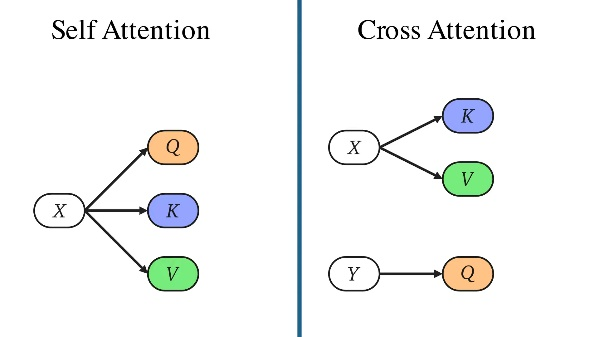
\includegraphics[width=0.60\textwidth]{./appunti_images/media/image89.jpeg}
\caption{Self-Attention vs Cross-Attention. Nella self-attention $Q,K,V$ vengono tutti dallo stesso input $X$. Nella cross-attention $K,V$ vengono dall'input $X$, mentre $Q$ viene da un altro array (i latenti $L$).}
\end{figure}

\begin{center}
\begin{tabular}{@{}lll@{}}
\toprule
\textbf{Aspetto} & \textbf{Transformer (Self-Att)} & \textbf{Perceiver (Cross-Att)} \\
\midrule
Sorgente $Q$        & Input $X$ ($M$ token)   & Latenti $L$ ($N$ latenti) \\
Sorgente $K, V$     & Input $X$ ($M$ token)   & Input $X$ ($M$ token) \\
Matrice attenzione  & $M \times M$ (quadrata) & $N \times M$ (rettangolare) \\
Complessità         & $O(M^2)$                & $O(MN)$, con $N \ll M$ \\
\bottomrule
\end{tabular}
\end{center}

\begin{notabox}[title={\textbf{Intuizione di $Q$, $K$, $V$}}]
\textbf{Query} $=$ una \emph{domanda} (``cosa sto cercando?''). \quad \textbf{Key} $=$ un'\emph{etichetta} (``io rappresento questo''). \quad \textbf{Value} $=$ il \emph{contenuto} informativo vero e proprio. L'attenzione confronta ogni domanda con tutte le etichette e restituisce una media pesata dei contenuti più pertinenti.
\end{notabox}

\begin{figure}[htbp]
\centering
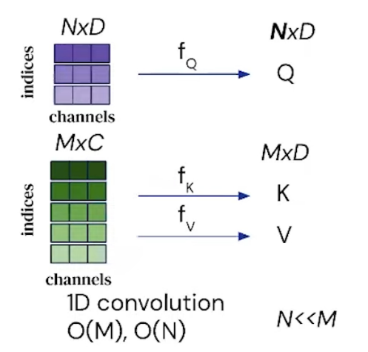
\includegraphics[width=0.46\textwidth]{./appunti_images/media/image44.png}
\caption{Cross-attention, primo step: il \emph{latent array} ($N \times D$) genera le Query $Q$, mentre il \emph{byte array} ($M \times C$) genera Key $K$ e Value $V$. Sono le \emph{sorgenti diverse} di $Q$ e di $K,V$ a definire la cross-attention.}
\end{figure}

I \textbf{latenti} $L$ sono \emph{parametri appresi} del modello (inizializzati come learned position encodings, paper App.~C): \textbf{non derivano dall'input} e non hanno un legame spaziale con pixel o token specifici. Sono una \emph{base compatta} --- delle ``unità di memoria'' --- che il modello usa per riassumere qualsiasi input.

\begin{ideabox}[title={\textbf{Idea chiave}}]
La cross-attention è un piccolo gruppo di $N$ latenti che ``\textbf{interroga}'' i $M$ elementi dell'input: $Q$ dai latenti (\emph{cosa cerco?}), $K/V$ dall'input (\emph{cosa contengo?}). L'asimmetria $N \ll M$ è ciò che rompe la quadraticità.
\end{ideabox}

% =====================================================================
\section{Architettura in tre stadi}
\stage{0}
% =====================================================================

\begin{brevebox}[title={\textbf{In breve}}]
Tre stadi: \textbf{(1)} un encoder a cross-attention \emph{comprime} l'input nei latenti; \textbf{(2)} un latent transformer \emph{raffina} i latenti con self-attention; \textbf{(3)} una testa di pooling $+$ classificatore produce i logit. Il blocco (1)$+$(2) si ripete $T$ volte.
\end{brevebox}

L'idea di fondo è \textbf{separare la dimensione dei dati in ingresso dalla capacità della rete}. Un input arbitrariamente grande viene prima proiettato in un latent array di dimensione fissa, e solo su quello la rete fa la sua elaborazione profonda. Ne discendono le due proprietà che \emph{definiscono} il Perceiver:

\begin{enumerate}
\item lo stesso modello gestisce modalità molto diverse \textbf{senza modifiche};
\item la \textbf{profondità della rete è disaccoppiata} dalla lunghezza dell'input.
\end{enumerate}

\begin{figure}[htbp]
\centering
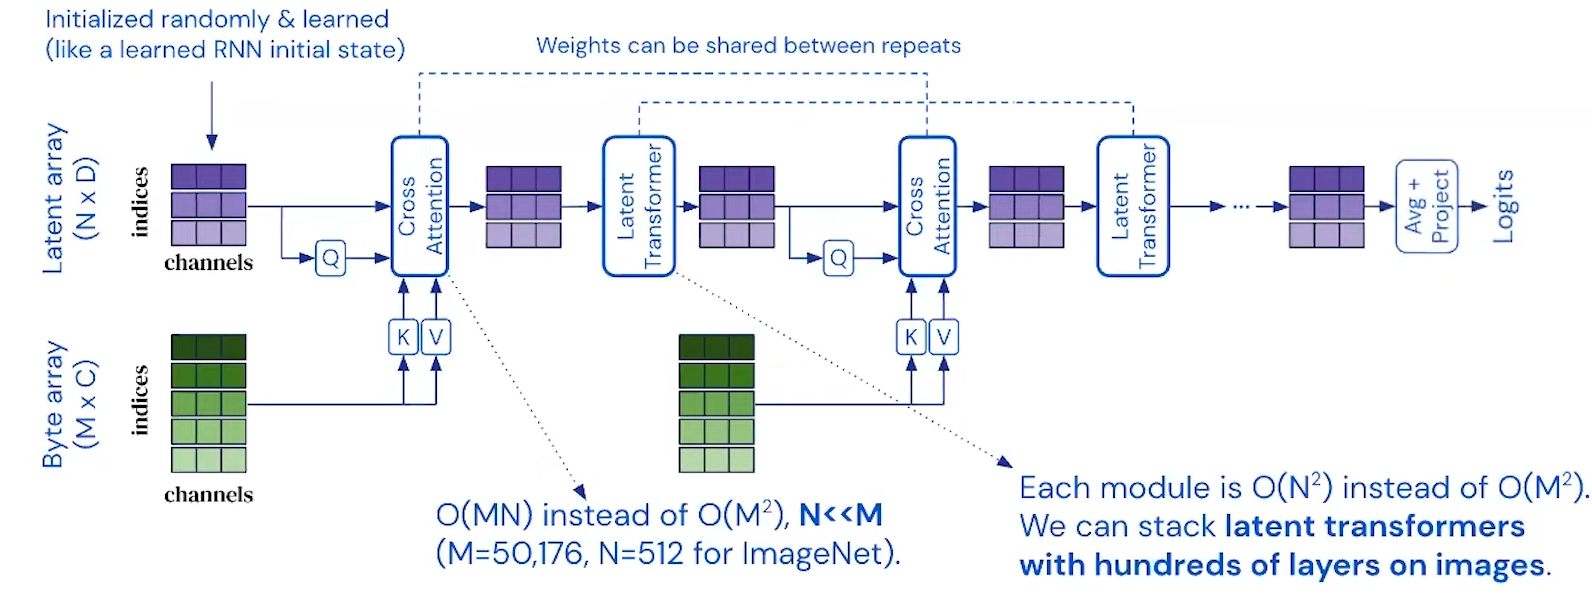
\includegraphics[width=0.92\textwidth]{./appunti_images/media/image47.png}
\caption{Architettura del Perceiver. Il \emph{Byte Array} ($M \times C$) entra da sinistra, viene letto dal \emph{Latent Array} ($N \times D$) tramite Cross-Attention, poi i latenti sono raffinati dal \emph{Latent Transformer}, infine mediati (Average $+$ Project) per produrre i \emph{Logits}. I pesi sono condivisi tra le $T$ iterazioni (linea tratteggiata in alto).}
\end{figure}

L'elaborazione si snoda in \textbf{tre stadi}:

\begin{enumerate}
\item \textbf{Encoder a cross-attention} --- legge l'input $X \in \mathbb{R}^{M \times C_{\text{tot}}}$ e lo \emph{comprime} nel latent array $L \in \mathbb{R}^{N \times D}$.
\item \textbf{Latent transformer} --- raffina $L$ con self-attention profonda, interamente nello spazio compresso.
\item \textbf{Testa di pooling $+$ classificazione} --- aggrega i latenti e produce i logit.
\end{enumerate}

Il blocco \emph{cross-attention $+$ latent transformer} viene poi ripetuto $T$ volte (con weight sharing, \S\ref{sec:ws}).

\begin{table}[htbp]
\centering
\caption{Iperparametri del Perceiver nella configurazione ImageNet (Jaegle et al., 2021, \S4.1 $+$ App.~C). Questi valori ricorrono in tutto il forward pass.}
\begin{tabular}{@{}lll@{}}
\toprule
\textbf{Simbolo} & \textbf{Valore} & \textbf{Significato} \\
\midrule
$M$               & $50\,176$  & elementi di input ($224\times224$ pixel) \\
$C$               & $3$        & canali grezzi (RGB) \\
$C_{\text{tot}}$  & $261$      & canali per elemento dopo le Fourier features \\
$N$               & $512$      & numero di latenti \quad ($N \ll M$) \\
$D$               & $1024$     & dimensione di ogni latente \\
$d_{QKV}$         & $261$      & dim.\ interna cross-attention $= \min(D, C_{\text{tot}})$ \\
$T$               & $8$        & iterazioni (cross-att $+$ latent transformer) \\
$\ell$            & $6$        & self-attention per blocco del latent transformer \\
$H$               & $8$        & teste della self-attention latente ($d_{\text{head}}=128$) \\
$K$               & $64$       & bande di frequenza Fourier per asse \\
\bottomrule
\end{tabular}
\end{table}

\begin{notabox}
\textbf{Cross-attention} (encoder): single-head nel paper, $d_{QKV} = \min(D, C_{\text{tot}}) = 261$. \quad
\textbf{Latent transformer}: self-attention multi-head, $H=8$ teste da $d_{\text{head}} = 128$.
\end{notabox}

% =====================================================================
\section{Il forward pass passo per passo}
\stage{0}
% =====================================================================

\begin{brevebox}[title={\textbf{In breve --- la pipeline}}]
\centering
Input $\to$ Fourier PE $\to$ Latent array $\to$ [\,Cross-Attention $\to$ Latent Transformer\,]$\times T$ $\to$ Pooling $\to$ Logits

\smallskip
\raggedright\small Ogni stadio è una sottosezione qui sotto. La \textbf{striscia in cima alla pagina} segue il tuo punto nella pipeline.
\end{brevebox}

Seguiamo i dati lungo tutta la pipeline, tracciando a ogni passo la \textbf{forma delle matrici} (esempi numerici per ImageNet).

% ---------------------------------------------------------------------
\subsection{Input: il byte array}
\stage{1}
% ---------------------------------------------------------------------

L'input grezzo --- qualunque esso sia --- viene ``appiattito'' in un \textbf{byte array} di forma $M \times C$: $M$ elementi, ciascuno con $C$ canali. È una \textbf{rappresentazione uniforme}: lo stesso formato per ogni modalità (è da qui che nasce la generalità del modello).

\begin{esempiobox}[title={\textbf{Esempio numerico --- immagine ImageNet}}]
Un'immagine RGB $224 \times 224$:
\begin{itemize}
\item numero di pixel: $M = 224 \times 224 = \mathbf{50\,176}$;
\item canali per pixel: $C = 3$ (R, G, B);
\item valori (byte) totali: $50\,176 \times 3 = \mathbf{150\,528}$.
\end{itemize}
La griglia di pixel viene linearizzata (\emph{reshape}) in una sequenza:
\[
\text{Byte Array} = [\,r_1, g_1, b_1,\; r_2, g_2, b_2,\; \ldots,\; r_{50176}, g_{50176}, b_{50176}\,] \;\Rightarrow\; X_{\text{grezzo}} \in \mathbb{R}^{50\,176 \times 3}
\]
\end{esempiobox}

\begin{figure}[htbp]
\centering
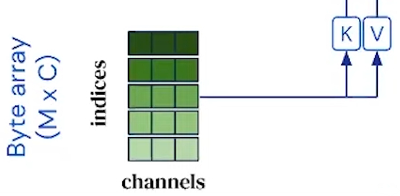
\includegraphics[width=0.42\textwidth]{./appunti_images/media/image52.png}
\caption{Il byte array ($M \times C$): ogni riga è un elemento dell'input (un pixel) con i suoi $C$ canali. Da qui si generano le Key e i Value della cross-attention.}
\end{figure}

Questo array però contiene solo il \emph{contenuto} (il colore dei pixel): \textbf{manca l'informazione di posizione}. Da solo, non distinguerebbe due immagini che differiscono per una semplice permutazione dei pixel.

\begin{center}
\small
\begin{tabular}{@{}llll@{}}
\toprule
\textbf{Oggetto} & \textbf{Forma simbolica} & \textbf{ImageNet} & \textbf{Contenuto di una riga} \\
\midrule
Byte array grezzo & $M \times C$ & $50\,176 \times 3$ & R, G, B di un pixel \\
\bottomrule
\end{tabular}
\end{center}

% ---------------------------------------------------------------------
\subsection{Positional encoding: le Fourier features}
\stage{2}
% ---------------------------------------------------------------------

\textbf{Problema:} l'attention è \emph{cieca alla posizione}. Un pixel $[R,G,B]$ dice solo il colore, non \emph{dove} si trova. Bisogna iniettare la posizione esplicitamente.

\textbf{Soluzione:} si arricchisce ogni elemento con le \textbf{Fourier features} --- la posizione $x$ viene mappata in uno spazio ad alta dimensione applicando seno e coseno a $K$ frequenze diverse.

\begin{formulabox}[title={\textbf{Fourier positional encoding}}]
Per ogni asse spaziale, dato il valore di coordinata $x_d \in [-1,1]$:
\[
\text{PE}(x_d) = \Big[\;\underbrace{\sin(f_1 \pi x_d),\,\cos(f_1 \pi x_d),\,\ldots,\,\sin(f_K \pi x_d),\,\cos(f_K \pi x_d)}_{2K\text{ valori sinusoidali}},\;\;\underbrace{x_d}_{\text{coord.\ grezza}}\;\Big]
\]
\end{formulabox}

\textbf{Tre scelte di design da ricordare:}

\begin{itemize}
\item \textbf{Frequenze \emph{linearly spaced}} tra $1$ e $\mu/2$ (la frequenza di Nyquist), \emph{non} esponenziali come in NeRF ($f_k = 2^k$). Con $K=64$ bande, NeRF darebbe $2^{64}\approx 10^{19}$: numeri ingestibili, e il paper riporta instabilità di training già oltre $k\approx15$ (App.~D).
\item \textbf{Si concatena anche la coordinata grezza} $x_d$: le sinusoidi sono \emph{periodiche} (quindi ambigue --- frequenze alte mappano posizioni diverse nello stesso valore), mentre la coordinata grezza dà l'\emph{identità} posizionale esatta.
\item \textbf{Si \emph{concatena}} al colore, non si \emph{somma}: la concatenazione tiene colore e posizione separati. (I Transformer per il linguaggio invece \emph{sommano} il positional encoding.)
\end{itemize}

\begin{esempiobox}[title={\textbf{Esempio numerico --- un pixel a posizione $(0.3,\,0.7)$}}]
Pixel rosso, posizione normalizzata $(x,y) = (0.3,\,0.7)$.
\begin{itemize}
\item Colore RGB normalizzato: $[1.0,\;0,\;0]$.
\item Fourier per l'asse $x = 0.3$, con 2 frequenze illustrative $f_1{=}1, f_2{=}2$ (il paper ne usa $64$):
\[
\text{PE}(0.3) = [\,\underbrace{0.3}_{x},\; \sin(0.3\pi),\; \cos(0.3\pi),\; \sin(0.6\pi),\; \cos(0.6\pi)\,]
            = [\,0.3,\; 0.809,\; 0.588,\; 0.951,\; -0.309\,]
\]
\item Analogamente per l'asse $y = 0.7$.
\item Vettore finale del pixel: $[\,\underbrace{1.0, 0, 0}_{\text{RGB}},\; \underbrace{0.3, \ldots}_{129\ (\text{asse }x)},\; \underbrace{0.7, \ldots}_{129\ (\text{asse }y)}\,] \in \mathbb{R}^{261}$.
\end{itemize}
\end{esempiobox}

\begin{formulabox}[title={\textbf{Da dove viene $C_{\text{tot}} = 261$}}]
Per ogni asse: $2K + 1 = 2{\cdot}64 + 1 = 129$ valori ($128$ sinusoidi $+$ $1$ coordinata grezza). \\
Con $d = 2$ assi (x e y): $2 \times 129 = 258$ valori posizionali. \\
Sommati ai $3$ canali RGB:
\[
C_{\text{tot}} = \underbrace{3}_{\text{RGB}} \;+\; \underbrace{d \times (2K+1)}_{2 \,\times\, 129 \;=\; 258 \text{ Fourier}} \;=\; \mathbf{261}
\]
\end{formulabox}

\begin{figure}[htbp]
\centering
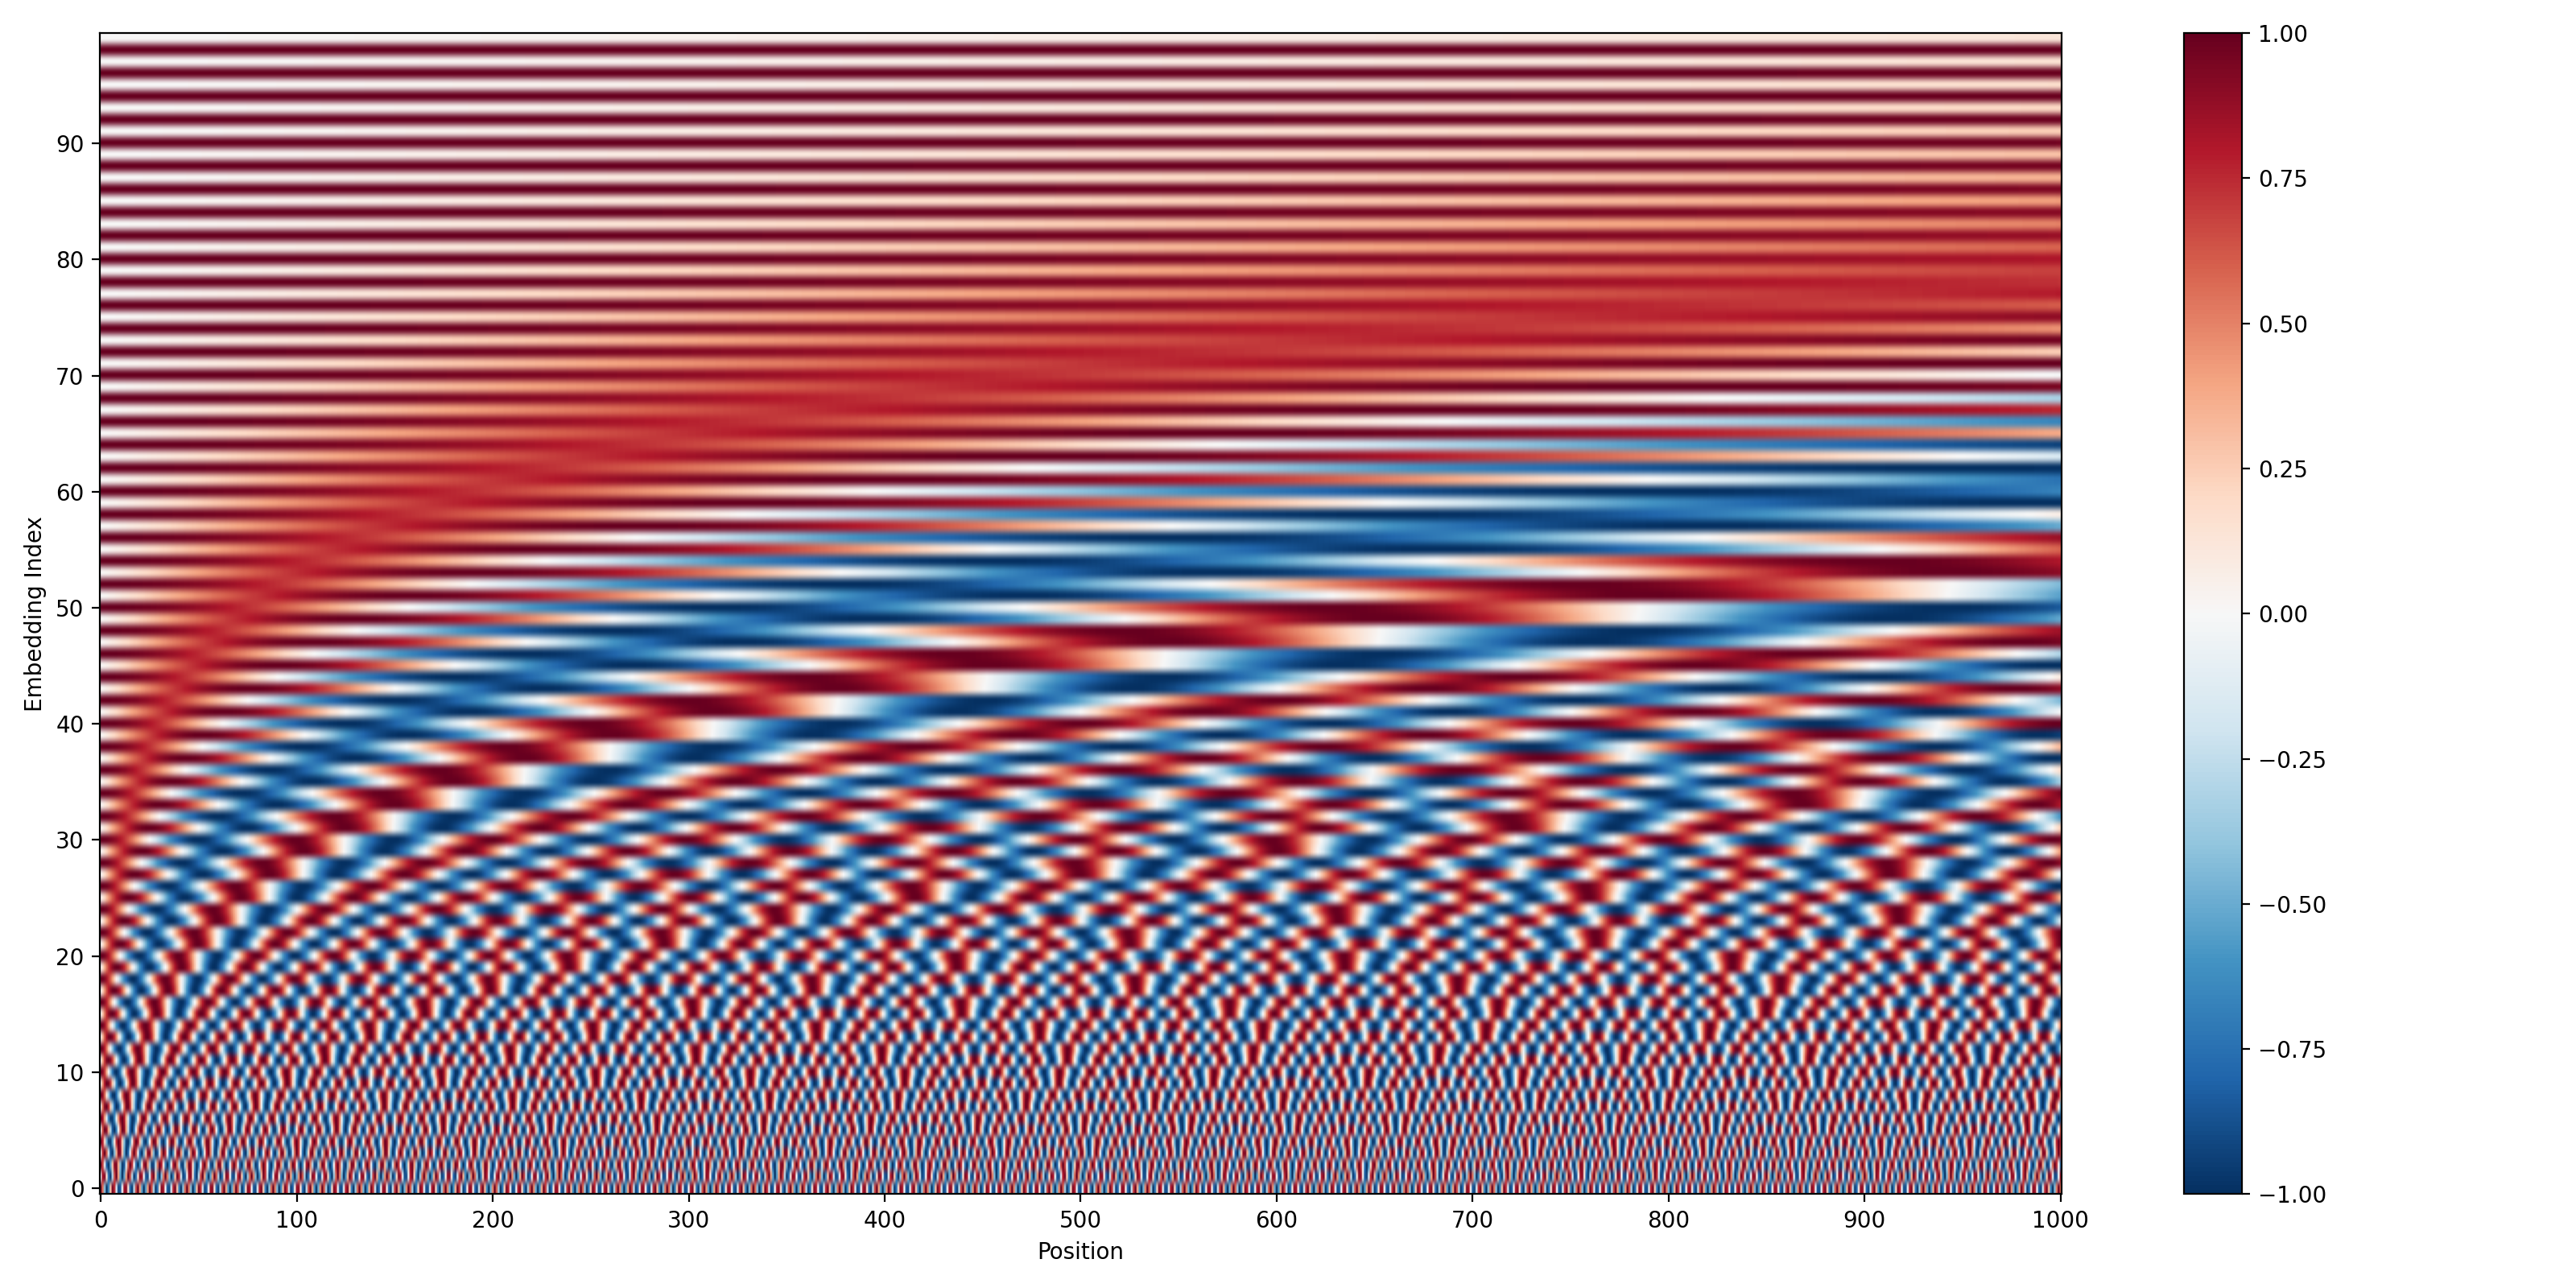
\includegraphics[width=0.62\textwidth]{./appunti_images/papers/fig_positional_encoding.png}
\caption{Le Fourier features mappano una posizione scalare in un vettore di sinusoidi a frequenze multiple: le basse frequenze catturano la posizione globale, le alte i dettagli fini.}
\end{figure}

\begin{center}
\small
\begin{tabular}{@{}llll@{}}
\toprule
\textbf{Oggetto} & \textbf{Forma simbolica} & \textbf{ImageNet} & \textbf{Contenuto di una riga} \\
\midrule
Byte array grezzo & $M \times C$ & $50\,176 \times 3$ & RGB \\
\textbf{Byte array $X$ (con Fourier PE)} & $\boldsymbol{M \times C_{\text{tot}}}$ & $\mathbf{50\,176 \times 261}$ & $3$ RGB $+$ $258$ Fourier \\
\bottomrule
\end{tabular}
\end{center}

\begin{ideabox}[title={\textbf{Idea chiave}}]
Le Fourier features danno al modello la \textbf{posizione}. È questa scelta --- non l'architettura in sé --- a rendere il Perceiver \textbf{invariante alle permutazioni} dei pixel: la posizione ``viaggia'' dentro l'input, non nell'ordine degli indici (vedi \S\ref{sec:risultati}).
\end{ideabox}

% ---------------------------------------------------------------------
\subsection{Il latent array}
\stage{3}
% ---------------------------------------------------------------------

Il \textbf{latent array} $L \in \mathbb{R}^{N \times D}$ è una matrice di $N$ vettori latenti, \textbf{interamente appresa} (sono parametri del modello). Non deriva dall'input: è uguale per tutti gli esempi del batch e cambia solo durante il training.

\begin{esempiobox}[title={\textbf{Inizializzazione dei latenti}}]
Per ImageNet $L \in \mathbb{R}^{512 \times 1024}$. Ogni elemento è campionato da una gaussiana stretta:
\[
L_{ij} \sim \mathcal{N}(0,\; 0.02^2), \qquad \text{troncata a } [-2,\,2].
\]
I valori sono quasi tutti minuscoli ($\sim\pm0.02$). \textbf{Perché così piccoli?}
\begin{itemize}
\item \textbf{Stabilità}: latenti grandi $\to$ prodotti $QK^\top$ enormi $\to$ softmax satura $\to$ gradienti instabili.
\item \textbf{Neutralità}: media zero $\Rightarrow$ nessun latente parte avvantaggiato.
\item \textbf{Specializzazione graduale}: partendo ``neutri'', i latenti si riempiono progressivamente di informazione e col tempo ciascuno si specializza (bordi, colori, pattern globali\dots).
\end{itemize}
\end{esempiobox}

\begin{figure}[htbp]
\centering
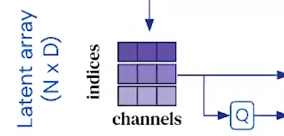
\includegraphics[width=0.42\textwidth]{./appunti_images/media/image60.png}
\caption{Il latent array ($N \times D$): matrice appresa che genera le Query ($Q$) per la cross-attention.}
\end{figure}

A questo punto abbiamo i \textbf{due array} che la cross-attention metterà in comunicazione:

\begin{center}
\small
\begin{tabular}{@{}llll@{}}
\toprule
\textbf{Oggetto} & \textbf{Forma} & \textbf{ImageNet} & \textbf{Natura} \\
\midrule
Byte array $X$            & $M \times C_{\text{tot}}$ & $50\,176 \times 261$ & input ($3$ RGB $+$ $258$ Fourier) \\
\textbf{Latent array} $\boldsymbol{L}$ & $\boldsymbol{N \times D}$ & $\mathbf{512 \times 1024}$ & parametri appresi, init $\mathcal{N}(0,0.02^2)$ \\
\bottomrule
\end{tabular}
\end{center}

Nota: i due array hanno dimensione-feature \emph{diversa} ($261$ vs $1024$); sarà la cross-attention a farli incontrare. E il numero di righe è molto diverso ($50\,176$ vs $512$): è questa asimmetria a dare la complessità $O(MN)$.

% ---------------------------------------------------------------------
\subsection{Il blocco di cross-attention}
\stage{4}
% ---------------------------------------------------------------------

Qui gli $N$ latenti ``leggono'' informazione dagli $M$ elementi dell'input. Vediamo i passaggi con le forme esatte.

\begin{figure}[htbp]
\centering
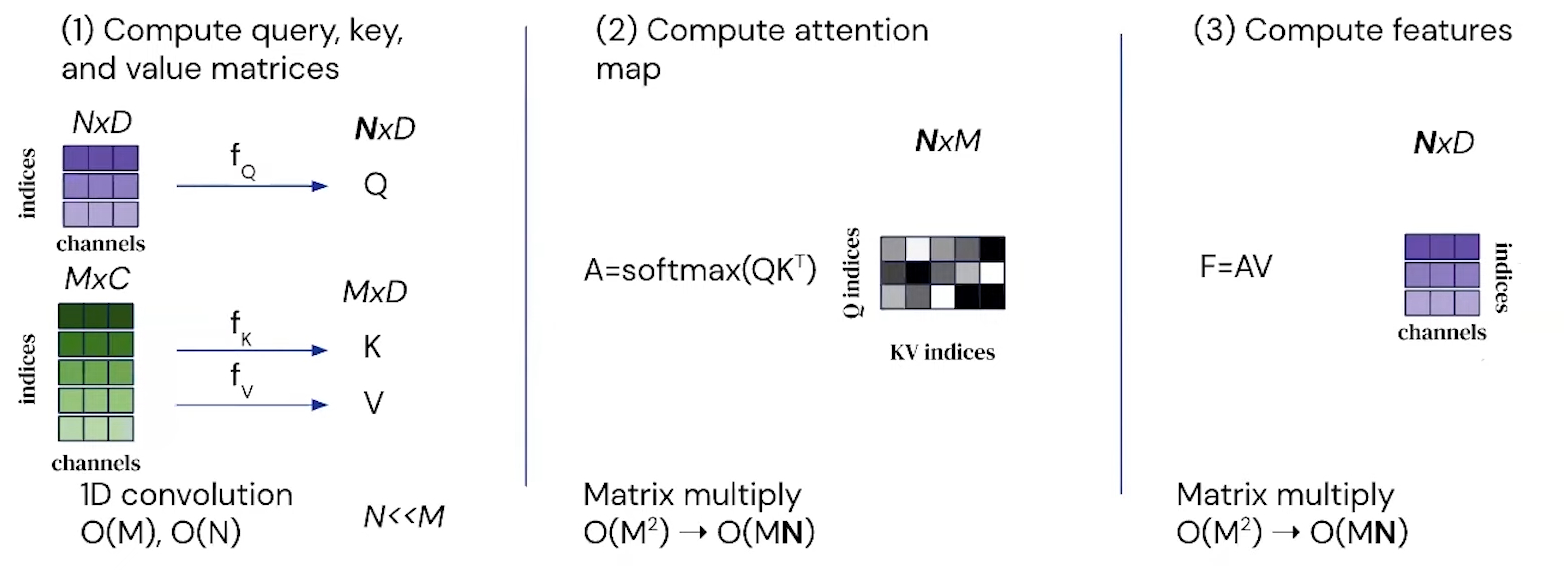
\includegraphics[width=0.80\textwidth]{./appunti_images/media/image43.png}
\caption{Cross-attention, vista d'insieme dei 3 step: (1) si calcolano le matrici $Q,K,V$; (2) si calcola la mappa di attenzione $N \times M$; (3) si aggregano le feature.}
\end{figure}

\textbf{Passo 1 --- LayerNorm pre-attention.} Entrambi gli array attraversano una \textbf{LayerNorm} prima delle proiezioni (pattern \emph{pre-norm}, paper App.~C). La LN normalizza \emph{ogni riga} a media $0$ e varianza $1$, poi applica due parametri appresi $\gamma,\beta$. Non cambia le forme: $\tilde X \in \mathbb{R}^{50\,176 \times 261}$, $\tilde L \in \mathbb{R}^{512 \times 1024}$.

\textit{Perché pre-norm?} Il residuo resta un percorso ``pulito'' su cui il gradiente fluisce senza attraversare la LN $\Rightarrow$ training stabile su reti profonde (lo stesso schema di GPT-2).

\textbf{Passo 2 --- dimensione interna $d_{QKV}$.} $Q,K,V$ devono avere la stessa dimensione-feature, altrimenti $QK^\top$ non è definito. Si sceglie:
\[
d_{QKV} = \min(D,\; C_{\text{tot}}) = \min(1024,\; 261) = \mathbf{261}.
\]
\textit{Perché il minimo?} L'input ha già solo $261$ canali: proiettare $K,V$ in una dimensione più grande non aggiungerebbe informazione, sarebbe solo spreco di parametri e FLOPs.

\textbf{Passo 3 --- proiezioni $Q$, $K$, $V$.} Tre matrici di pesi apprese (\emph{senza bias}, paper App.~C):

\begin{formulabox}[title={\textbf{Proiezioni lineari}}]
\[
\begin{array}{lll}
Q = \tilde L\, W_Q, & W_Q \in \mathbb{R}^{D \times d_{QKV}} = \mathbb{R}^{1024 \times 261}, & Q \in \mathbb{R}^{512 \times 261} \quad(\text{dai latenti})\\[3pt]
K = \tilde X\, W_K, & W_K \in \mathbb{R}^{C_{\text{tot}} \times d_{QKV}} = \mathbb{R}^{261 \times 261}, & K \in \mathbb{R}^{50\,176 \times 261} \quad(\text{dall'input})\\[3pt]
V = \tilde X\, W_V, & W_V \in \mathbb{R}^{C_{\text{tot}} \times d_{QKV}} = \mathbb{R}^{261 \times 261}, & V \in \mathbb{R}^{50\,176 \times 261} \quad(\text{dall'input})
\end{array}
\]
\end{formulabox}

Le matrici $W_Q, W_K, W_V$ sono \emph{apprese}: imparano a produrre query, key e value ``ottimali'' per il matching (es.\ riducendo il peso di feature rumorose). I pesi sono inizializzati con \emph{Xavier Uniform} (Glorot \& Bengio, 2010), che mantiene costante la varianza delle attivazioni attraverso i layer. \textbf{L'asimmetria chiave}: $Q$ ha \emph{poche} righe ($N=512$), $K,V$ ne hanno \emph{tante} ($M=50\,176$).

\textbf{Passo 4 --- scaled dot-product attention.} Le quattro operazioni che combinano $Q,K,V$:

\begin{figure}[htbp]
\centering
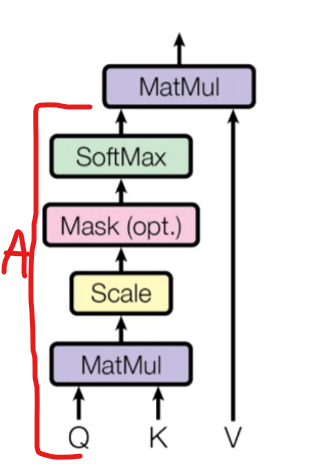
\includegraphics[width=0.40\textwidth]{./appunti_images/media/image63.png}
\caption{Pipeline della scaled dot-product attention: prodotto $QK^\top$, scaling per $\sqrt{d_{QKV}}$, softmax per riga, prodotto finale con $V$. (Il passo ``Mask'' non è usato: il Perceiver è non-causale.)}
\end{figure}

\begin{formulabox}[title={\textbf{Scaled dot-product}}]
\[
\begin{array}{ll}
\text{(a) score} & S = QK^\top \in \mathbb{R}^{512 \times 50\,176} \\[3pt]
\text{(b) scaling} & S' = S / \sqrt{d_{QKV}} = S/\sqrt{261} \approx S/16 \\[3pt]
\text{(c) softmax per riga} & A_{ij} = e^{S'_{ij}} \big/ \textstyle\sum_{k=1}^{M} e^{S'_{ik}}, \qquad A \in \mathbb{R}^{512 \times 50\,176} \\[6pt]
\text{(d) aggregazione} & F = A\,V \in \mathbb{R}^{512 \times 261}
\end{array}
\]
\end{formulabox}

\begin{itemize}
\item \textbf{(a)} ogni entry $(i,j)$ misura ``quanto il latente $i$ trova interessante il pixel $j$''.
\item \textbf{(b)} senza scaling gli score avrebbero deviazione standard $\sqrt{d_{QKV}}\approx16$: la softmax saturerebbe (tutta la massa su un pixel) e i gradienti si annullerebbero.
\item \textbf{(c)} la softmax rende i pesi non-negativi e con somma $1$ su ogni riga $\Rightarrow$ ogni latente ha un ``budget di attenzione'' da distribuire sui $50\,176$ pixel.
\item \textbf{(d)} ogni latente diventa una \emph{media pesata} dei Value dell'input.
\end{itemize}

\begin{figure}[htbp]
\centering
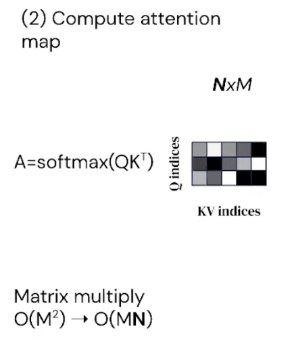
\includegraphics[width=0.34\textwidth]{./appunti_images/media/image45.png}
\caption{La mappa di attenzione $A = \text{softmax}(QK^\top/\sqrt{d_{QKV}})$ è \textbf{rettangolare} $N \times M = 512 \times 50\,176$ (righe $=$ latenti, colonne $=$ pixel) --- non quadrata $M \times M$. È qui che la complessità scende da $O(M^2)$ a $O(MN)$.}
\end{figure}

\textbf{Passo 5 --- output projection e residual.} $F$ vive in dimensione $261$; va riportato a $D=1024$ per poterlo sommare ai latenti:
\[
Z' = F\,W_o + b_o, \quad W_o \in \mathbb{R}^{261 \times 1024} \;\Rightarrow\; Z' \in \mathbb{R}^{512 \times 1024};
\qquad L' = L + Z' \in \mathbb{R}^{512 \times 1024}.
\]

\textbf{Passo 6 --- MLP (feed-forward).} Pre-norm, espansione a $4D$, attivazione GELU, compressione, residual:
\[
\tilde L' = \text{LN}(L'); \quad
H = \tilde L'\,W_1 + b_1 \in \mathbb{R}^{512 \times 4096}; \quad
\phi = \text{GELU}(H)\,W_2 + b_2 \in \mathbb{R}^{512 \times 1024}; \quad
\hat L = L' + \phi.
\]

\begin{figure}[htbp]
\centering
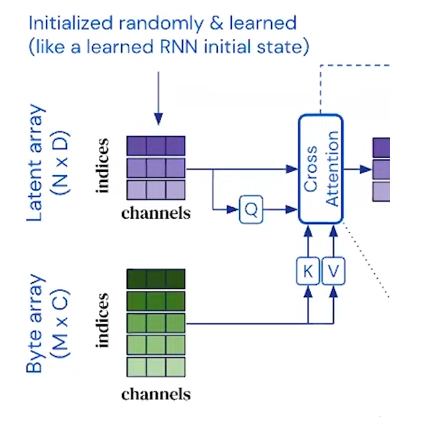
\includegraphics[width=0.55\textwidth]{./appunti_images/media/image62.png}
\caption{Schema complessivo della cross-attention: il latent array ($512 \times 1024$) proiettato a $Q$ ($512 \times 261$) interroga il byte array ($50\,176 \times 261$) proiettato a $K,V$. Il prodotto $QK^\top$ dà una matrice di attenzione rettangolare $512 \times 50\,176$.}
\end{figure}

\begin{table}[htbp]
\centering
\caption{Riepilogo completo del blocco Cross-Attention $+$ MLP (ImageNet). Input: $L \in \mathbb{R}^{512\times1024}$, $X \in \mathbb{R}^{50\,176\times261}$.}
\small
\renewcommand{\arraystretch}{1.25}
\begin{tabular}{@{}clll@{}}
\toprule
\textbf{\#} & \textbf{Operazione} & \textbf{Formula} & \textbf{Dimensione} \\
\midrule
\multicolumn{4}{@{}l@{}}{\emph{\textbf{Cross-Attention}}} \\
1 & LayerNorm pre-att. & $\tilde L = \text{LN}(L),\;\; \tilde X = \text{LN}(X)$ & invariate \\
2 & Proiezione $Q$ & $Q = \tilde L\,W_Q,\;\; W_Q \in \mathbb{R}^{1024 \times 261}$ & $\mathbb{R}^{512 \times 261}$ \\
  & Proiezione $K$ & $K = \tilde X\,W_K,\;\; W_K \in \mathbb{R}^{261 \times 261}$ & $\mathbb{R}^{50\,176 \times 261}$ \\
  & Proiezione $V$ & $V = \tilde X\,W_V,\;\; W_V \in \mathbb{R}^{261 \times 261}$ & $\mathbb{R}^{50\,176 \times 261}$ \\
3 & Scaled scores & $S = QK^\top / \sqrt{261}$ & $\mathbb{R}^{512 \times 50\,176}$ \\
4 & Softmax per riga & $A_{ij} = e^{S_{ij}} / \sum_k e^{S_{ik}}$ & $\mathbb{R}^{512 \times 50\,176}$ \\
5 & Aggregazione & $F = A\,V$ & $\mathbb{R}^{512 \times 261}$ \\
6 & Output projection & $Z' = F\,W_o + b_o,\;\; W_o \in \mathbb{R}^{261 \times 1024}$ & $\mathbb{R}^{512 \times 1024}$ \\
7 & Residual & $L' = L + Z'$ & $\mathbb{R}^{512 \times 1024}$ \\
\midrule
\multicolumn{4}{@{}l@{}}{\emph{\textbf{MLP} (pre-norm, GELU, hidden $4D$)}} \\
8  & LayerNorm pre-MLP & $\tilde L' = \text{LN}(L')$ & $\mathbb{R}^{512 \times 1024}$ \\
9  & Espansione $+$ GELU & $H' = \text{GELU}(\tilde L'\,W_1 + b_1),\; W_1 \in \mathbb{R}^{1024 \times 4096}$ & $\mathbb{R}^{512 \times 4096}$ \\
   & Compressione & $\phi = H'\,W_2 + b_2,\;\; W_2 \in \mathbb{R}^{4096 \times 1024}$ & $\mathbb{R}^{512 \times 1024}$ \\
10 & Residual post-MLP & $\hat L = L' + \phi$ & $\mathbb{R}^{512 \times 1024}$ \\
\bottomrule
\end{tabular}
\end{table}

\begin{ideabox}[title={\textbf{Idea chiave}}]
Output del blocco: $\hat L \in \mathbb{R}^{512 \times 1024}$, \textbf{stessa forma di $L$}. Il blocco non cambia la dimensione del latent array, solo il suo \emph{contenuto} --- ora arricchito dell'informazione letta dall'input. È questa invarianza di forma che permette di ripetere il blocco $T$ volte.
\end{ideabox}

% ---------------------------------------------------------------------
\subsection{Il latent transformer}
\stage{5}
% ---------------------------------------------------------------------

Una volta che i latenti contengono l'informazione, vengono \textbf{raffinati} da una pila di $\ell$ blocchi di \textbf{self-attention} che operano \emph{solo sui latenti} ($N \times D$), senza più toccare l'input. Qui i latenti ``comunicano tra loro'': è il passo che \emph{integra} l'informazione raccolta dalla cross-attention.

\begin{figure}[htbp]
\centering
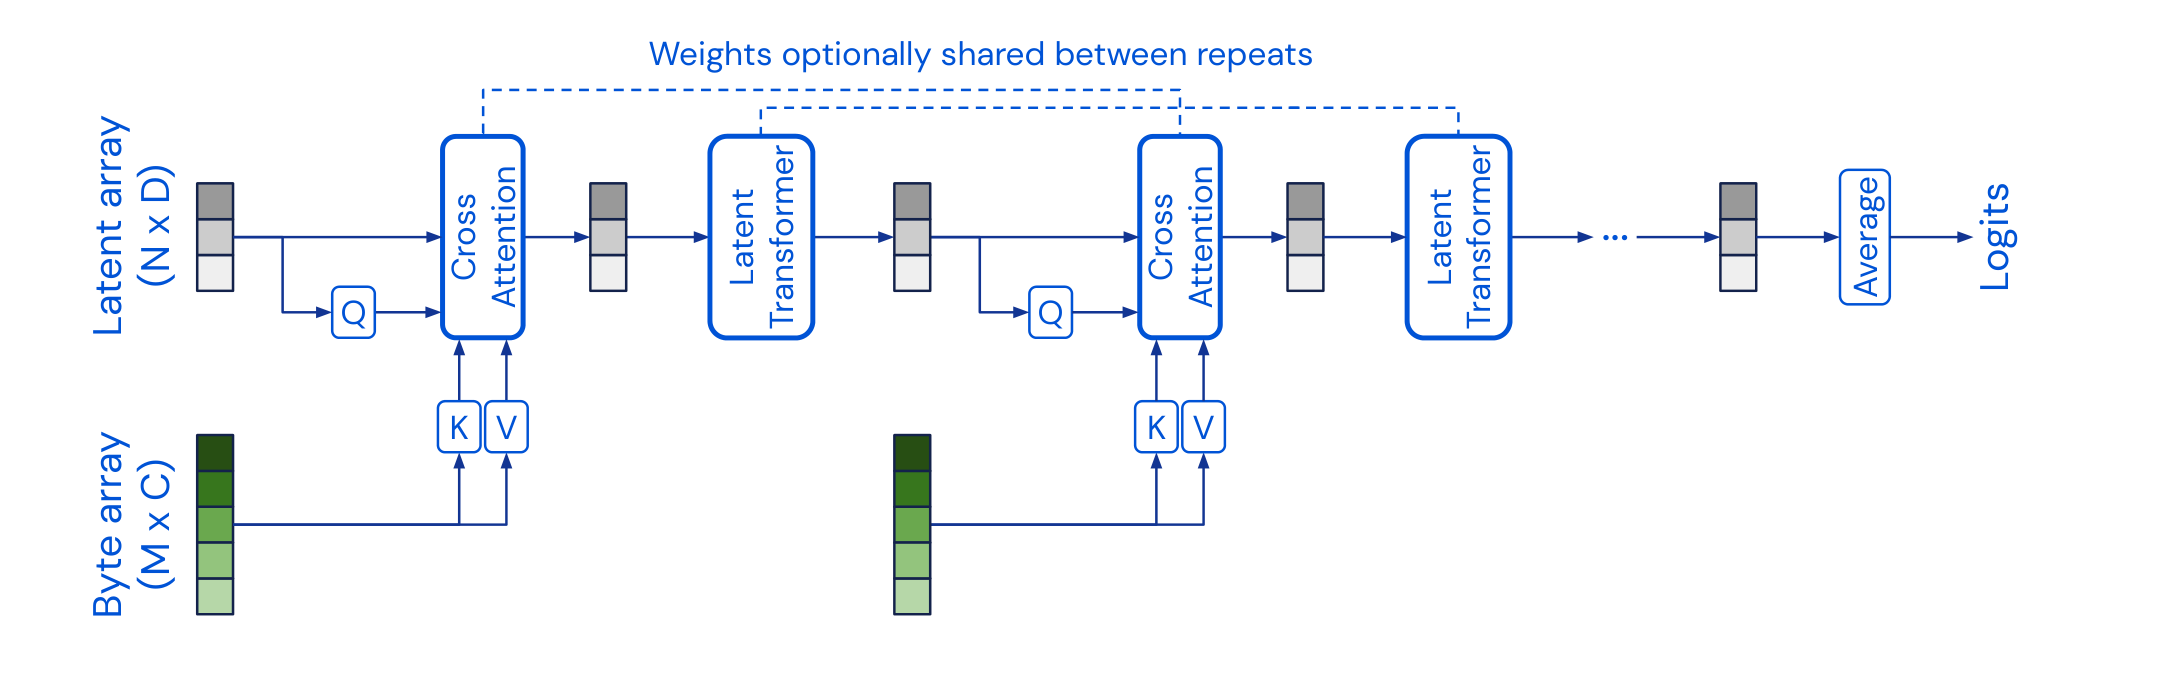
\includegraphics[width=0.92\textwidth]{./appunti_images/papers/perceiver_orig_fig1_full.png}
\caption{Il latent transformer nella pipeline del Perceiver (Jaegle et al., 2021, Fig.~1): si alterna alla cross-attention e opera \emph{solo} sui latenti tramite self-attention profonda.}
\end{figure}

Struttura di un blocco (architettura \textbf{GPT-2}, Radford et al., 2019): LayerNorm $\to$ multi-head self-attention $\to$ residual $\to$ LayerNorm $\to$ MLP (GELU, hidden $4D$) $\to$ residual. Non causale --- nessuna maschera.

\textbf{Self-attention multi-head} ($H = 8$ teste, $d_{\text{head}} = D/H = 128$). Qui $Q,K,V$ vengono \emph{tutti} dai latenti:
\[
Q = \tilde L\,W_q,\;\; K = \tilde L\,W_k,\;\; V = \tilde L\,W_v \quad(W \in \mathbb{R}^{1024 \times 128}\text{ per testa});
\qquad A = \text{softmax}\!\Big(\tfrac{QK^\top}{\sqrt{d_{\text{head}}}}\Big) \in \mathbb{R}^{512 \times 512}.
\]

I risultati delle $8$ teste vengono concatenati ($512 \times 1024$) e proiettati da $W_O$.

\begin{notabox}[title={\textbf{Multi-head: perché più teste?}}]
Invece di una sola attention in dimensione $D$, se ne calcolano $H$ in parallelo, ciascuna in dimensione $d_{\text{head}} = D/H$. Ogni testa può specializzarsi su un tipo di relazione diverso (es.\ una guarda pattern locali, un'altra globali). I risultati si concatenano: il costo totale resta lo stesso di una singola attention in dimensione $D$.
\end{notabox}

\begin{center}
\small
\begin{tabular}{@{}lll@{}}
\toprule
\textbf{Aspetto} & \textbf{Cross-attention} & \textbf{Latent transformer} \\
\midrule
Sorgente $Q$        & latenti              & latenti \\
Sorgente $K,V$      & \textbf{input} $X$   & \textbf{latenti} \\
Tipo                & cross-attention      & self-attention \\
Dim.\ interna       & $d_{QKV}=261$        & $D=1024$ ($8$ teste da $128$) \\
Matrice attenzione  & $512 \times 50\,176$ (rettangolare) & $512 \times 512$ (quadrata) \\
Costo               & $O(MN)$              & $O(N^2)$ --- piccolo grazie al bottleneck \\
\bottomrule
\end{tabular}
\end{center}

\begin{ideabox}[title={\textbf{Idea chiave}}]
La \textbf{profondità} del modello vive qui, nello spazio latente compresso. La matrice di attenzione è $N \times N = 512 \times 512$: impilare molti layer costa $O(N^2)$, \emph{non} $O(M^2)$. Ecco perché la profondità della rete è \textbf{disaccoppiata} dalla dimensione dell'input.
\end{ideabox}

% ---------------------------------------------------------------------
\subsection{Weight sharing e iterazioni}
\label{sec:ws}
\stage{6}
% ---------------------------------------------------------------------

È una delle idee più importanti del Perceiver. Il blocco \emph{cross-attention $+$ latent transformer} viene riapplicato $\mathbf{T = 8}$ volte agli stessi latenti, \textbf{condividendo i pesi} tra le iterazioni --- con un'eccezione: il \emph{primo} blocco ha pesi propri.

\begin{notabox}[title={\textbf{Perché il primo blocco è escluso dallo sharing}}]
La prima cross-attention riceve i latenti nella loro inizializzazione ``neutra'' ($\mathcal{N}(0,0.02^2)$); dalla seconda in poi legge invece latenti già ``popolati'' di informazione. Due regimi così diversi non possono condividere gli stessi pesi senza causare \textbf{instabilità di training}. Quindi $\text{CA}_1, \text{LT}_1$ hanno pesi unici; $\text{CA}_2,\ldots,\text{CA}_T$ e $\text{LT}_2,\ldots,\text{LT}_T$ condividono ciascuno un set di pesi.
\end{notabox}

\begin{figure}[htbp]
\centering
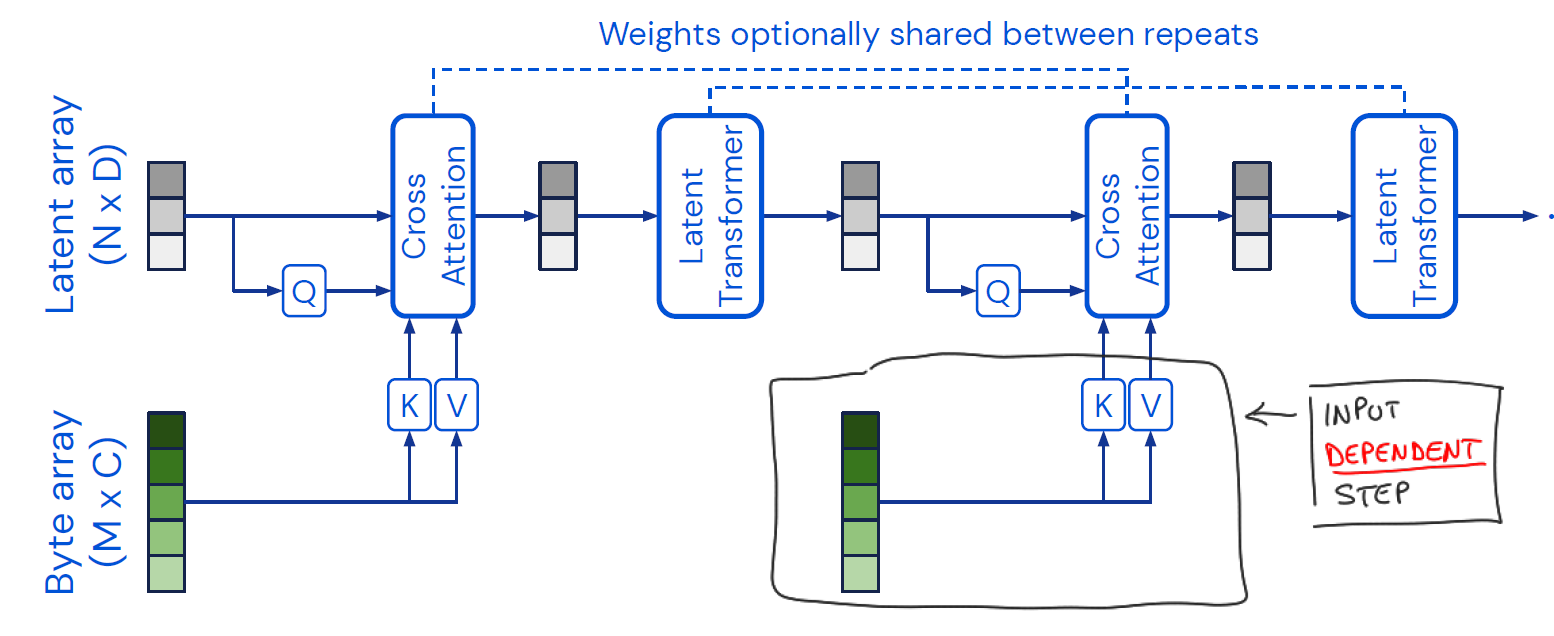
\includegraphics[width=0.82\textwidth]{./appunti_images/media/image75.png}
\caption{Il Perceiver completo con weight sharing (Jaegle et al., 2021, Fig.~1): i blocchi Cross-Attention e Latent Transformer si ripetono $T$ volte condividendo i pesi (linee tratteggiate).}
\end{figure}

Questo rende il Perceiver \textbf{formalmente un RNN}:

\begin{center}
\small
\begin{tabular}{@{}ll@{}}
\toprule
\textbf{Componente RNN} & \textbf{Nel Perceiver} \\
\midrule
stato ricorrente        & il latent array $L^{(t)}$ (dimensione fissa $512 \times 1024$) \\
input (costante nel tempo) & il byte array $X$ \\
funzione di transizione & il blocco condiviso (cross-att $+$ latent transformer) \\
stato iniziale          & $L^{(0)}$ (parametro appreso) \\
\bottomrule
\end{tabular}
\end{center}

A differenza di un RNN classico, però, a \emph{ogni} passo i latenti accedono all'\textbf{intero input simultaneamente}, non a un elemento alla volta.

\begin{esempiobox}[title={\textbf{Esempio numerico --- gradienti di un peso condiviso}}]
Sia $w = 2.0$ un peso condiviso tra le iterazioni $t=2$ e $t=3$. Nel backward ogni istanza produce un contributo:
\[
\frac{\partial \mathcal{L}}{\partial w^{(2)}} = -0.3, \qquad \frac{\partial \mathcal{L}}{\partial w^{(3)}} = +0.1.
\]
I contributi si \textbf{sommano} (come in un RNN srotolato --- BPTT):
\[
\frac{\partial \mathcal{L}}{\partial w^{\text{sh}}} = -0.3 + 0.1 = -0.2.
\]
Con learning rate $\eta = 0.01$: \;$w \leftarrow w - \eta \cdot (-0.2) = 2.0 + 0.002 = \mathbf{2.002}$.

\smallskip
\emph{Attenzione}: l'accumulazione va fatta \emph{prima} del passo dell'ottimizzatore. In PyTorch è automatica (più nodi del grafo che puntano allo stesso \texttt{Parameter}).
\end{esempiobox}

\begin{formulabox}[title={\textbf{Effetto del weight sharing (Tab.~7 del paper)}}]
\begin{tabular}{@{}lll@{}}
\textbf{Senza} weight sharing: & $\sim$326M parametri & $72.9\%$ accuracy (forte overfitting) \\
\textbf{Con} weight sharing:   & $\sim$45M parametri  & $\mathbf{78.0\%}$ accuracy \\
\end{tabular}

\smallskip
$\Rightarrow$ $\sim$\textbf{7$\times$ meno parametri} \emph{e contemporaneamente} $\mathbf{+5.1\%}$ di accuracy.
\end{formulabox}

\begin{ideabox}[title={\textbf{Idea chiave}}]
Il weight sharing trasforma il Perceiver in un RNN che \textbf{raffina progressivamente} i latenti, rileggendo l'input $T$ volte con lo stesso ``modulo di raffinamento''. Agisce da \textbf{regolarizzatore}: meno parametri, niente overfitting, più accuratezza.
\end{ideabox}

% ---------------------------------------------------------------------
\subsection{Output: pooling e classificazione}
\stage{7}
% ---------------------------------------------------------------------

Dopo le $T$ iterazioni, dai latenti finali $L^{(T)} \in \mathbb{R}^{512 \times 1024}$ si arriva alla predizione in tre passi.

\begin{figure}[htbp]
\centering
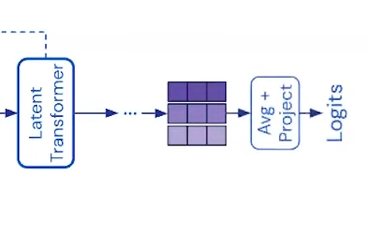
\includegraphics[width=0.50\textwidth]{./appunti_images/media/image76.png}
\caption{Testa di output: i latenti finali vengono mediati (Average) e proiettati (Project) nei logit per la classificazione.}
\end{figure}

\begin{esempiobox}[title={\textbf{Dai latenti alla classe predetta (ImageNet, 1000 classi)}}]
\textbf{1. Global average pooling} --- media degli $N$ latenti finali:
\[
h = \frac{1}{N}\sum_{i=1}^{N} L_i^{(T)} \;\in\; \mathbb{R}^{D} = \mathbb{R}^{1024}.
\]
\textbf{2. Classificatore lineare} --- proietta nello spazio delle classi:
\[
z = h\,W_c + b_c, \qquad W_c \in \mathbb{R}^{1024 \times 1000},\; b_c \in \mathbb{R}^{1000} \;\Rightarrow\; z \in \mathbb{R}^{1000}\ \text{(logit)}.
\]
\textbf{3. Softmax $+$ argmax} --- logit $\to$ probabilità $\to$ classe:
\[
p_i = \frac{e^{z_i}}{\sum_{j=1}^{1000} e^{z_j}}, \qquad \hat y = \arg\max_i p_i.
\]
\end{esempiobox}

A differenza di BERT/GPT, il Perceiver \textbf{non usa un token \texttt{[CLS]}}: il pooling medio è la soluzione più diretta e \emph{non introduce nuovi parametri}. Il pooling è fatto \emph{prima} della proiezione lineare (un fix del paper, App.~F).

\begin{ideabox}[title={\textbf{Idea chiave}}]
Il pooling medio comprime gli $N$ latenti in \emph{un solo} vettore $h \in \mathbb{R}^D$, di dimensione fissa --- qualunque sia $N$. Questo permette di collegare un classificatore lineare standard, identico per qualsiasi modalità di input.
\end{ideabox}

\begin{notabox}[title={\textbf{E il backward pass?}}]
Il modello è allenato end-to-end con la \emph{backpropagation} standard applicata a ogni blocco. Con il weight sharing, i gradienti dei blocchi condivisi si \textbf{sommano} prima del passo dell'ottimizzatore (come in un RNN srotolato --- BPTT, vedi esempio in \S\ref{sec:ws}). La derivazione completa dei gradienti è meccanica e non introduce concetti teorici nuovi: per la \emph{teoria} del Perceiver basta la pipeline forward qui sopra.
\end{notabox}

% =====================================================================
\section{I componenti ricorrenti}
\stage{0}
% =====================================================================

\begin{brevebox}[title={\textbf{In breve}}]
Il Perceiver riusa quattro ``mattoni'' standard del deep learning: \textbf{LayerNorm} (normalizza), \textbf{GELU} (la non-linearità delle MLP), la \textbf{residual connection} (la somma $x + f(x)$) e la \textbf{softmax} (da punteggi a probabilità). Compaiono in \emph{ogni} blocco del forward pass.
\end{brevebox}

Il Perceiver non introduce nuovi ``pezzi'' a basso livello: la sua novità sta nell'\emph{architettura} (cross-attention, latent bottleneck, weight sharing), non nei singoli componenti. Questi ultimi sono quattro elementi standard che conviene conoscere bene, perché ricorrono in tutta la pipeline.

\subsection{LayerNorm --- normalizzazione}

La \textbf{Layer Normalization} stabilizza la distribuzione dei valori che entrano in attention e MLP. Agisce \emph{riga per riga}: per ogni elemento (un latente, o un pixel) $x = (x_1,\ldots,x_F)$ calcola media $\mu$ e deviazione standard $\sigma$ delle sue $F$ feature, e applica:
\[
\hat x_j = \gamma_j \cdot \frac{x_j - \mu}{\sigma + \epsilon} + \beta_j .
\]
Prima si normalizza a media $0$ e varianza $1$ (\emph{per costruzione matematica}); poi due parametri \emph{appresi} per-feature, $\gamma$ (scala) e $\beta$ (shift), lasciano alla rete la libertà di ri-tarare la distribuzione. Il termine $\epsilon \approx 10^{-5}$ evita la divisione per zero.

\textbf{Pre-norm.} Il Perceiver applica la LayerNorm \emph{prima} di ogni sotto-blocco, non dopo: $y = x + f(\text{LN}(x))$. Così il ramo residuo resta un percorso ``pulito'' su cui il gradiente scorre senza attraversare la LN $\Rightarrow$ training stabile anche con molti layer. Una LN precede \emph{ogni} cross-attention, \emph{ogni} self-attention e \emph{ogni} MLP.

\begin{figure}[htbp]
\centering
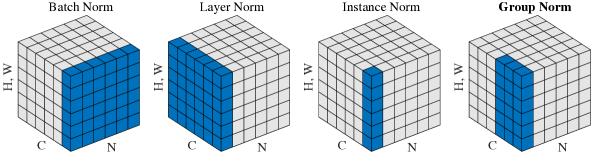
\includegraphics[width=0.72\textwidth]{./appunti_images/papers/fig_normalization_methods.png}
\caption{Metodi di normalizzazione a confronto. Il Perceiver usa la \textbf{LayerNorm}, che normalizza lungo le feature di \emph{ogni singolo elemento} --- indipendentemente dagli altri esempi del batch.}
\end{figure}

\subsection{GELU --- la funzione di attivazione}

Dentro ogni \textbf{MLP} serve una \emph{non-linearità}: senza, due layer lineari in sequenza collasserebbero in uno solo e la rete non potrebbe imparare funzioni complesse. Il Perceiver usa la \textbf{GELU} (Gaussian Error Linear Unit):
\[
\text{GELU}(x) = x \cdot \Phi(x),
\]
dove $\Phi$ è la funzione di ripartizione della gaussiana standard: in pratica ogni valore viene pesato per la ``probabilità di essere grande''.

\textbf{GELU vs ReLU.} La ReLU azzera di colpo tutti i valori negativi (un ``gomito'' netto in $0$); la GELU è \emph{liscia}, lascia passare una piccola parte dei valori leggermente negativi ed è differenziabile ovunque. La transizione morbida rende l'ottimizzazione più stabile. Il Perceiver adotta la GELU seguendo l'architettura GPT-2/BERT.

\begin{figure}[htbp]
\centering
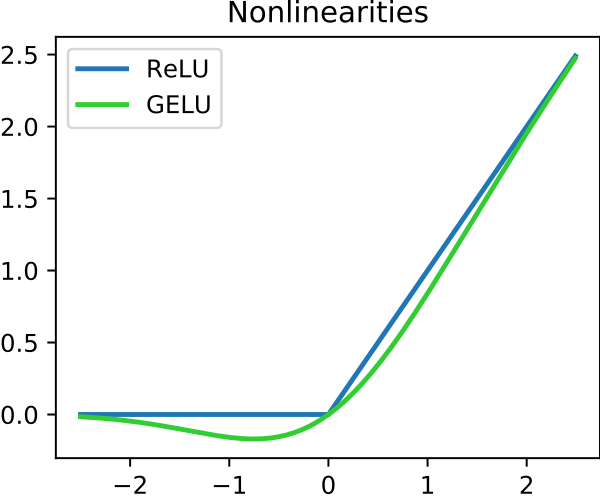
\includegraphics[width=0.50\textwidth]{./appunti_images/papers/fig_relu_gelu.png}
\caption{ReLU vs GELU. La ReLU ha un gomito netto in $0$; la GELU è liscia e lascia passare leggermente i valori negativi vicini a zero.}
\end{figure}

\subsection{Residual connection --- la somma che salva il gradiente}

Una \textbf{residual connection} (o \emph{skip connection}) trasforma un blocco da $\text{output} = f(x)$ a:
\[
\text{output} = x + f(x),
\]
cioè \textbf{somma l'input} al risultato del blocco. Sembra un dettaglio, ma è ciò che rende addestrabili le reti \emph{profonde}: nel backward il gradiente trova un \textbf{percorso diretto} attraverso il ``$+$'' (la derivata della somma rispetto a $x$ contiene un $1$), quindi non si attenua strato dopo strato --- niente \emph{vanishing gradient}. È l'idea che ha reso possibili le ResNet.

Nel Perceiver \emph{ogni} sotto-blocco è avvolto in una residual: $L' = L + \text{Attention}(\text{LN}(L))$ e poi $\hat L = L' + \text{MLP}(\text{LN}(L'))$. Insieme al pre-norm, è ciò che permette di impilare in profondità il latent transformer.

\begin{figure}[htbp]
\centering
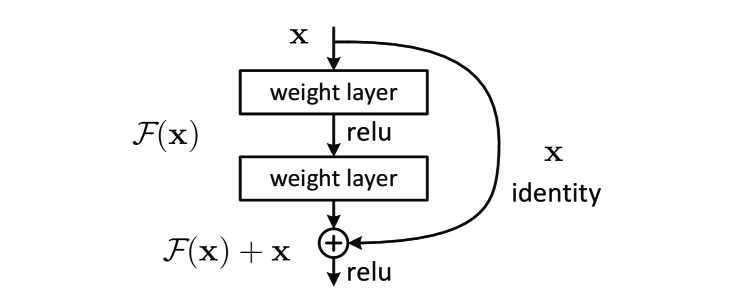
\includegraphics[width=0.42\textwidth]{./appunti_images/papers/fig_residual_block.png}
\caption{Un blocco residuale: l'input $x$ ``salta'' il blocco $f$ e viene sommato alla sua uscita. Il ramo diretto è una corsia preferenziale per il gradiente.}
\end{figure}

\subsection{Softmax --- da punteggi a probabilità}

La \textbf{softmax} trasforma un vettore di numeri reali qualsiasi (i \emph{punteggi}) in una \textbf{distribuzione di probabilità}:
\[
\text{softmax}(z)_i = \frac{e^{z_i}}{\sum_{j} e^{z_j}} .
\]
Le sue proprietà: tutti i valori finiscono in $[0,1]$, \textbf{sommano a $1$}, l'ordine dei punteggi è preservato e i valori più grandi vengono enfatizzati (per via dell'esponenziale).

Nel Perceiver la softmax compare \textbf{due volte}: \textbf{(1)} nella \emph{mappa di attenzione}, applicata riga per riga --- ogni latente ottiene una distribuzione di pesi sui pixel (un ``budget di attenzione'' che somma a $1$); \textbf{(2)} alla \emph{fine}, sui logit, per ottenere le probabilità delle classi. Nei calcoli reali si sottrae prima il massimo di ogni riga, per evitare overflow numerico (trucco \emph{log-sum-exp}), senza cambiare il risultato.

\begin{figure}[htbp]
\centering
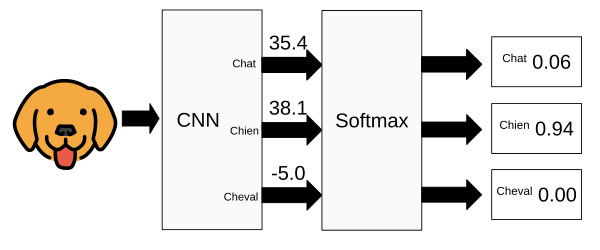
\includegraphics[width=0.55\textwidth]{./appunti_images/papers/fig_softmax.png}
\caption{La softmax converte un vettore di punteggi arbitrari in una distribuzione di probabilità: valori non-negativi che sommano a $1$.}
\end{figure}

\begin{ideabox}[title={\textbf{Idea chiave}}]
La forza del Perceiver non sta in componenti esotici --- usa gli stessi mattoni di un Transformer qualunque --- ma in \emph{come} li dispone: cross-attention con latenti, bottleneck, weight sharing. Una volta chiari questi quattro mattoni, ogni formula del forward pass diventa trasparente.
\end{ideabox}

% =====================================================================
\section{Dettagli di training (ImageNet)}
\stage{0}
% =====================================================================

\begin{brevebox}[title={\textbf{In breve}}]
Training su ImageNet: ottimizzatore \textbf{LAMB}, $120$ epoche, learning rate con \emph{step decay}, \textbf{niente dropout}, $\sim$45M parametri (come una ResNet).
\end{brevebox}

\begin{notabox}
\begin{itemize}
\item \textbf{Ottimizzatore}: LAMB (You et al., 2020). Il paper riporta che il Perceiver è più facile da ottimizzare con LAMB che con Adam.
\item \textbf{Schedule}: $120$ epoche; learning rate iniziale $4\times10^{-3}$ con \emph{step decay} ($\div10$ alle epoche $84/102/114$). Niente cosine, niente warmup.
\item \textbf{No dropout}: il paper lo ha provato e ha osservato un \emph{peggioramento} (App.~C). Il modello ha già forti pressioni regolarizzanti --- bottleneck $N \ll M$, weight sharing, weight decay, data augmentation aggressiva (RandAugment, Cubuk et al., 2020).
\item \textbf{Dimensione}: $\sim$45M parametri, paragonabile a una ResNet usata su ImageNet.
\end{itemize}
\end{notabox}

% =====================================================================
\section{Risultati chiave}
\label{sec:risultati}
\stage{0}
% =====================================================================

\begin{brevebox}[title={\textbf{In breve}}]
\textbf{ImageNet 78.0\%} su pixel grezzi, senza convoluzioni 2D --- alla pari di ResNet-50 e ViT. \textbf{Permutation invariance}: $78.0 \to 78.0$ sotto permutazione dei pixel, \emph{zero} calo. È il risultato che dimostra la vera generalità del modello.
\end{brevebox}

\textbf{Classificazione ImageNet} (top-1, pixel grezzi). Il Perceiver raggiunge $\mathbf{78.0\%}$ lavorando direttamente sui $50\,176$ pixel \emph{senza convoluzioni 2D}.

\begin{table}[htbp]
\centering
\caption{ImageNet top-1 accuracy (validation), Tab.~1 del paper. FF $=$ Fourier features.}
\small
\begin{tabular}{@{}lcl@{}}
\toprule
\textbf{Modello} & \textbf{Top-1 (val)} & \textbf{Note} \\
\midrule
ResNet-50                  & $77.6\%$ & convoluzioni 2D \\
ViT-B/16                   & $77.9\%$ & patch 2D \\
Transformer ($64{\times}64$, FF) & $57.0\%$ & input downsamplato (costretto da $O(M^2)$) \\
\textbf{Perceiver (FF)}    & $\mathbf{78.0\%}$ & $50\,176$ pixel grezzi, \textbf{nessuna conv 2D} \\
\bottomrule
\end{tabular}
\end{table}

È competitivo con ResNet-50 e ViT-B/16, entrambi con un forte \emph{prior} 2D. Il Transformer puro fallisce ($57.0\%$): la complessità $O(M^2)$ lo costringe a downsamplare a $64\times64$, perdendo dettaglio.

\textbf{Permutation invariance --- il risultato chiave.} I pixel di tutte le immagini vengono mescolati con la \emph{stessa} permutazione fissa. Un modello che codifica la posizione \emph{nell'input} (via Fourier features) dovrebbe esserne immune.

\begin{table}[htbp]
\centering
\caption{ImageNet \emph{raw} vs \emph{permuted} (Tab.~2 del paper).}
\small
\begin{tabular}{@{}lcc@{}}
\toprule
\textbf{Modello} & \textbf{ImageNet \emph{raw}} & \textbf{ImageNet \emph{permuted}} \\
\midrule
\textbf{Perceiver} (Fourier features)  & \textbf{78.0} & \textbf{78.0} \\
Perceiver (learned position encoding)  & 78.0          & 70.9 \\
ViT-B/16 (FF)                          & 76.7          & 61.7 \\
ResNet-50 (FF)                         & 73.5          & 39.4 \\
\bottomrule
\end{tabular}
\end{table}

\begin{ideabox}[title={\textbf{Idea chiave --- il risultato che ``vende'' il Perceiver}}]
Il Perceiver con Fourier features è \textbf{invariante alla permutazione}: $78.0 \to 78.0$, zero calo. La ResNet crolla ($73.5 \to 39.4$) perché la conv 2D \emph{assume} che i vicini nella griglia siano correlati. Importante: la versione con \emph{learned} position encoding scende a $70.9$ $\Rightarrow$ è la scelta delle \textbf{Fourier features}, non l'architettura in sé, a dare l'invarianza. Il paper usa questo per argomentare che il Perceiver \emph{non} sfrutta un bias 2D nascosto: è davvero general-purpose.
\end{ideabox}

\textbf{Altri domini.} AudioSet (audio$+$video grezzi): $\sim$43\% mAP. ModelNet-40 (point cloud): $85.7\%$ contro il $91.9\%$ di PointNet++ --- il gap si spiega perché il Perceiver usa solo le coordinate $(x,y,z)$ grezze, senza feature geometriche specializzate. Conferma comunque la generalità dell'architettura.

% =====================================================================
\section{Ablation: cosa conta davvero}
\stage{0}
% =====================================================================

\begin{brevebox}[title={\textbf{In breve}}]
\textbf{Latent transformer} essenziale: senza, l'accuracy crolla a $\le 45\%$. \textbf{Weight sharing}: $7\times$ meno parametri e $+5.1\%$ di accuracy. \textbf{Cross-attention interleaved} (alternata) batte ``at-start'' (tutte all'inizio).
\end{brevebox}

Sintesi degli ablation studies del paper (App.~B, Figure 5--6, Tabelle 5--7).

\begin{table}[htbp]
\centering
\caption{I tre ablation più importanti: ogni componente, da sola, è essenziale.}
\small
\begin{tabular}{@{}lccl@{}}
\toprule
\textbf{Componente} & \textbf{Senza} & \textbf{Con (modello completo)} & \textbf{Conclusione} \\
\midrule
Latent transformer        & $\le 45\%$ (o OOM) & $78.0\%$ & il bottleneck è essenziale \\
Weight sharing            & $72.9\%$ ($326$M) & $78.0\%$ ($45$M) & regolarizzatore potente \\
Cross-att.\ \emph{interleaved} & $73.7\%$ (\emph{at-start}) & $78.0\%$ (\emph{interleaved}) & rileggere l'input conta \\
\bottomrule
\end{tabular}
\end{table}

\begin{itemize}
\item \textbf{Il latent bottleneck è essenziale.} Rimuovendo il latent transformer e usando solo cross-attention ripetute, l'accuracy crolla a $\le 45\%$ (o va in out-of-memory). Il bottleneck non è solo risparmio computazionale: è il \emph{meccanismo} che integra l'informazione globale tra i latenti.
\item \textbf{Interleaved $>$ at-start.} $8$ cross-attention \emph{alternate} al processo latente $\to 78.0\%$; le stesse $8$ tutte all'inizio $\to 73.7\%$. Il modello deve \textbf{ri-leggere} l'input più volte, con latenti progressivamente raffinati.
\item \textbf{Weight sharing $=$ regolarizzatore.} $\sim$7$\times$ meno parametri, $+5.1\%$ di accuracy, overfitting eliminato (gap train/val da $-14.8\%$ a $-1.5\%$).
\item \textbf{Fourier features.} Più bande di frequenza migliorano le prestazioni \textbf{fino alla frequenza di Nyquist}; oltre, nessun guadagno (sono ridondanti).
\item \textbf{$N$, $D$, $\ell$.} Aumentarli aiuta, ma $D$ oltre un certo punto causa overfitting --- mitigato proprio dal weight sharing.
\end{itemize}

\begin{esamebox}[title={\textbf{Da ricordare per l'esame}}]
\begin{itemize}\setlist{itemsep=3pt}
\item \textbf{Problema}: la self-attention costa $O(M^2)$ $\Rightarrow$ \textbf{soluzione}: latent bottleneck $N \ll M$, costo $O(MN) + O(N^2)$.
\item \textbf{Cross-attention}: $Q$ dai latenti, $K/V$ dall'input $\Rightarrow$ matrice di attenzione \emph{rettangolare} $N \times M$. Dim.\ interna $d_{QKV} = \min(D, C_{\text{tot}}) = 261$.
\item \textbf{Tre stadi}: encoder cross-attention $\to$ latent transformer (self-attention, architettura GPT-2) $\to$ pooling $+$ classificatore.
\item \textbf{Forme chiave (ImageNet)}: $X$ è $50\,176{\times}261$, $L$ è $512{\times}1024$, attenzione cross $512{\times}50\,176$, attenzione latente $512{\times}512$.
\item \textbf{Fourier PE}: frequenze \emph{linearly spaced} (no NeRF), si \emph{concatena} (no somma) $+$ coordinata grezza $\Rightarrow$ \textbf{permutation invariance}.
\item \textbf{Weight sharing}: il modello diventa un RNN; $7\times$ meno parametri, $+5.1\%$ accuracy.
\item \textbf{Numeri}: ImageNet $78.0\%$ (Fourier, senza conv 2D); \emph{permuted} $78.0\%$ (invariante); weight sharing $326$M$\to$45M parametri, $72.9\%\to78.0\%$.
\item \textbf{Training}: ottimizzatore LAMB, \emph{no} dropout, $\sim$45M parametri.
\end{itemize}
\end{esamebox}

% =====================================================================
\section*{Riferimenti}
\addcontentsline{toc}{section}{Riferimenti}
\stage{0}
% =====================================================================

\begin{notabox}
\textbf{Paper di riferimento}
\begin{itemize}\setlength\itemsep{0.15em}
\item \textbf{Jaegle, A.\ et al.\ (2021).} \emph{Perceiver: General Perception with Iterative Attention.} ICML 2021. --- il paper su cui si basa questo documento.
\item Vaswani, A.\ et al.\ (2017). \emph{Attention Is All You Need.} NeurIPS. --- Transformer e scaled dot-product attention.
\item Radford, A.\ et al.\ (2019). \emph{Language Models are Unsupervised Multitask Learners.} --- architettura GPT-2, usata nel latent transformer.
\item Mildenhall, B.\ et al.\ (2020). \emph{NeRF.} --- Fourier features con frequenze esponenziali (l'alternativa scartata).
\item Glorot, X.\ \& Bengio, Y.\ (2010). --- inizializzazione Xavier dei pesi.
\item You, Y.\ et al.\ (2020). \emph{LAMB.} --- ottimizzatore usato per il training su ImageNet.
\item Cubuk, E.\ et al.\ (2020). \emph{RandAugment.} --- data augmentation usata nel training.
\end{itemize}

\medskip
\textbf{Appendici del paper Perceiver (Jaegle et al., 2021) --- mappa rapida}
\begin{itemize}\setlength\itemsep{0.15em}
\item \textbf{App.\ B} --- Ablations: Tabelle 5--7 (weight sharing, cross-attends), Figure 5--6 (effetto di $N, D, \ell, T$).
\item \textbf{App.\ C} --- Dettagli architetturali: LayerNorm pre-norm, cross-attention single-head, $d_{QKV}=261$, no bias in $Q/K/V$, no dropout, init latenti $\mathcal{N}(0, 0.02^2)$.
\item \textbf{App.\ D} --- Positional encoding: frequenze linearly spaced tra $1$ e $\mu/2$, confronto esplicito con NeRF.
\item \textbf{App.\ F} --- Modifiche rispetto alla prima versione: rimozione del dropout, pooling \emph{prima} della proiezione.
\end{itemize}
\end{notabox}

\end{document}
